\documentclass{beamer}
\usetheme{Boadilla}
\usepackage{graphicx}
\usepackage{url}
\usepackage{multicol}
\graphicspath{ {images/} }

\title{Optimizing programs for smaller binary footprint}
\subtitle{}
\author{Alexander Livenets}
\institute{}
\date{\today}

\begin{document}

\AtBeginSection[]
{
  \begin{frame}
    \frametitle{Table of Contents}
    \tableofcontents[currentsection]
  \end{frame}
}

\begin{frame}
\titlepage
\end{frame}

\section{Introduction}

\subsection{Motivation}
\begin{frame}
\frametitle{\subsecname}
	\begin{itemize}
		\item Smaller boot-up time
		\item Better performance (in some cases)
		\item Faster image update
		\item Bootloaders, bare metal: smaller footprint, more space for user data and Rich OS
	\end{itemize}
\end{frame}

\subsection{Drawbacks}
\begin{frame}
\frametitle{\subsecname}
	\begin{itemize}
		\item Increased compilation time
		\item Some corner cases where optimization may fail
	\end{itemize}
\end{frame}

\section{Strategies}
\subsection{Yocto level}
\begin{frame}
\frametitle{System minification}
	\begin{itemize}
		\item Yocto build: In Release Yocto build, disable docs, includes, cmake modules
		\item Locales and fonts: cut them out, you ain't gonna need much in console, live with C UTF8 locale and one single font
		\item Strip binaries
		\item ARM: use hard FP instead of soft FP
		\item G++: Use newer compilers
		\item Libc: Use smaller libc alternatives (eglibc, bionic, musl, uclibc, newlib) (Licensing!)
		\item Clang: Compile with clang and libc++ for middleware and application services
		\item CMake: CMAKE\_BUILD\_TYPE=MinSizeRel
		\item Kernel: cut out unused modules (network, wifi,...)
		\item Kernel: build tiny kernel: \url{https://tiny.wiki.kernel.org/}
		\item Libraries: Analyze used libraries and components, cut out unused libraries (e.g. some of Qt), use single library for one function Examples (e.g. JSON, XML parsing, HTTP, etc.)
	\end{itemize}
\end{frame}

\begin{frame}
\frametitle{Data minification}
	\begin{itemize}
		\item Minify/compress scripts and markup/configuration files (JSON, XML, HTML, CSS, JavaScript)
		\item Compress images (PNG, SVG) - additional time to load them!
		\item Compile QML sources into one binary/library
	\end{itemize}
\end{frame}

\subsection{Service level}

\subsubsection{Compilation at a glance}

\begin{frame}
\frametitle{Compilation at a glance}
	\centering
	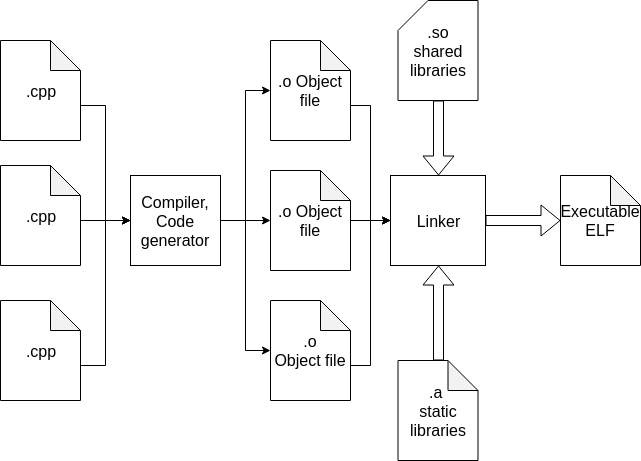
\includegraphics[scale=0.35]{CompilationDiagram.png}
\end{frame}

\begin{frame}
\frametitle{Compilation at a glance}
	\begin{itemize}
		\item .text - compiled code
		\item .rodata - variable initialization data + constants + strings
		\item .data - all global and static variables
		\item .bss - Better Save Space, zero-initialized variables
	\end{itemize}

	\centering
	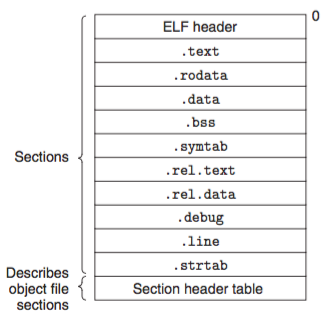
\includegraphics[scale=0.35]{RelocatedObject.png}
\end{frame}

\subsubsection{Compile-time feature toggle}

\begin{frame}
\frametitle{\subsubsecname}
	\begin{multicols}{2}
% \begin{verbatim}
% 		main.cpp

% 		#ifdef FEATURE
% 		class FeatureImpl {
% 		//...	
% 		};

% 		#endif

% 		int main(void) {
% 		#ifdef FEATURE
% 			registerFeature(new FeatureImpl());
% 		endif
% 			//other code...
% 		}
% \end{verbatim}
% \begin{verbatim}
% 		CMakeLists.txt:
% 		option(FEATURE ``Some feature'' ON)
% 		$ cmake .. -DFEATURE=OFF
% \end{verbatim}
	\end{multicols}
\end{frame}

\subsubsection{Compilation options}
\begin{frame}
\frametitle{\subsubsecname}
\begin{itemize}
	\item -Os - smaller and (maybe) faster than -O3 
	\item -s - strip resulting binary object in gcc
	\item -mtune - use CPU-specific compiler optimizations. Enables usage of extended CPU instruction set
	\item -fno-unroll-loops - do not unroll loops, may produce less code.
	\item -fno-inline-small-functions -finline-functions-called-once - optimization of inline functions, inline in certain cases
	\item -fshort-enums – shrink enums size to max contained value; WARNING: may break ABI (USE ONLY for static binaries)
\end{itemize}
\end{frame}

\subsubsection{Link options}
\begin{frame}
\frametitle{\subsubsecname}
\begin{itemize}
\item -ffunction-sections -fdata-sections to the compiler while building and -Wl,--gc-sections to the linker. Every function and variable goes to its own section, then they are optimized and glued (up to 30\% improvement)
\item strip --strip-all on the final executable (up to 20\% improvement)
\item -flto – LTO, link-time optimization, allows to optimize code across multiple object files
\item strip --remove-section=.comment –remove-section=.note, removing many copies of garbage strings like "GCC: (GNU) 4.0.1 20050727 (Red Hat 4.0.1-5)"
\end{itemize}
\end{frame}

\subsubsection{Code refactoring}
\begin{frame}
\frametitle{\subsubsecname}
\begin{itemize}
    \item Static vs. dynamic linking
    \begin{itemize} 
    	\item Static libraries: better, if used by one application. 
    	\item Split functions to source files, the resulting binary will be smaller and better optimized (great example: static libc and similar). 
    	\item WARNING: use static linking with caution, since it may cause undefined behavior and program crashes when used incorrectly
    	\item Dynamic libraries: less code size if used by multiple applications
	\end{itemize}
    \item Link only used libraries
    \item Logging! Logging creates a lot of strings. Some strings are quite similar:
% \begin{verbatim}
% $ strings AudioManager
%  ...
%  DBusWrapper::DBusWrapper DBus Connection is null
%  DBusWrapper::DBusWrapper DBus Connection is
%  ...
%  DBusWrapper::DBusWrapper Registering of watch functions failed
%  DBusWrapper::DBusWrapper Registering of timer functions failed
% \end{verbatim}
\end{itemize}
\end{frame}

\begin{frame}
\frametitle{\subsubsecname}
\begin{itemize}
    \item struct,class alignment and packing
    \item Less using C++ Templates, causing code bloat
    \item Don’t use C++ Exceptions, Compiler: -fno-exceptions
    \item Don’t use C++ RTTI, Compiler: -fno-rtti
    \item Pay attention to inline functions, causing code bloat
    \item Statically initialized large arrays and objects with custom (nonzero) data. They usually go to .text block. The initialization will happen anyway: before main or after, so, use it wisely (also applies for statically initialized C++ objects)
% \begin{verbatim}
%     static const std::vector<T> -> static const T[]
%     static const std::string -> static const char*
% \end{verbatim}
\end{itemize}
\end{frame}

\subsubsection{Compression}
\begin{frame}
\frametitle{\subsubsecname}
UPX: \url{https://upx.github.io} - in-place decompression of compressed executable/library
\end{frame}

\subsubsection{Disable optimization}
\begin{frame}
\frametitle{\subsubsecname}
\begin{itemize}
	\item \texttt{volatile} keyword
	\item \texttt{\#pragma GCC optimize(``O0'')}
\end{itemize}
\end{frame}

\section{Real-life example}
\begin{frame}
\frametitle{\secname}
GENIVI AudioManager: \url{https://github.com/GENIVI/AudioManager.git}

Fork with experiments: \url{https://github.com/alivenets/AudioManager.git}

Machine configuration: Intel Core-i7, x86\_64-linux-gnu, gcc 7.4.0, clang 6.0.0

GCC:
\begin{itemize} 
\item \texttt{cmake .. -DWITH\_CAPI\_WRAPPER=OFF -DWITH\_DBUS\_WRAPPER=ON} 
\item Compiler-specific optimization flags: \texttt{-fno-unroll-loops -fno-inline-small-functions -finline-functions-called-once}
\end{itemize}
Clang: 
\begin{itemize}
\item \texttt{CC=/usr/bin/clang CXX=/usr/bin/clang++ cmake .. -DCMAKE\_USER\_MAKE\_RULES\_OVERRIDE=\$(pwd)/../ClangDefinitions.txt -DWITH\_CAPI\_WRAPPER=OFF -DWITH\_DBUS\_WRAPPER=ON}
\item Compiler-specific optimization flags: \texttt{-fvectorize}
\end{itemize}

Libraries are linked statically!
\end{frame}


\begin{frame}
\frametitle{\secname}

\begin{table}\small
% \resizebox{\linewidth}{!}
\begin{tabular}{ccccccll}
\cline{1-5}
\multicolumn{1}{l}{Release (-O2)} & \multicolumn{1}{l}{MinSizeRel (-Os)} & \multicolumn{1}{l}{-march=corei7} & \multicolumn{1}{l}{Section GC flags} & \multicolumn{1}{l}{Misc flags} & \multicolumn{1}{l}{LTO} & Clang                                                                          & Gcc                                                                           \\ \cline{1-5}
V                                 &                                      &                                   &                                      &                                &                         & \begin{tabular}[c]{@{}l@{}}1020K (not stripped)\\ 780K (stripped)\end{tabular} & \begin{tabular}[c]{@{}l@{}}1.1M (not stripped)\\ 819K (stripped)\end{tabular} \\
                                  & V                                    &                                   &                                      &                                &                         & \begin{tabular}[c]{@{}l@{}}1.1M (not stripped)\\ 764K (stripped)\end{tabular}  & \begin{tabular}[c]{@{}l@{}}947K (not stripped)\\ 651K (stripped)\end{tabular} \\
                                  & V                                    & V                                 &                                      &                                &                         & 764K (stripped)                                                                & 651K (stripped)                                                               \\ \cline{1-5}
                                  & V                                    & V                                 & V                                    &                                &                         & 764K (stripped)                                                                & 651K (stripped)                                                               \\
                                  & V                                    & V                                 & V                                    & V                              &                         & 764K (stripped)                                                                & 651K (stripped)                                                               \\
                                  & V                                    &                                   &                                      &                                & V                       & FAILED                                                                         & 499K (stripped)                                                               \\
                                  & V                                    & V                                 & V                                    & V                              & V                       & FAILED                                                                         & 487K (stripped)                                                              
\end{tabular}
\end{table}
\end{frame}

\section{Further research}
\begin{frame}
\frametitle{\secname}
\begin{itemize}
	    \item Yocto tinification on real example
    \item Test on Aarch64 architecture
    \item Run optimization for current Yocto image
    \item Clang LTO + advanced optimization research
\end{itemize}
\end{frame}

\section{Resources}
\begin{frame}
\frametitle{\secname}
\tiny

Executable size reduction techniques in Linux

\begin{itemize}
\item \url{https://wiki.wxwidgets.org/Reducing_Executable_Size}
\item \url{http://www.catch22.net/tuts/win32/reducing-executable-size}
\item \url{http://ptspts.blogspot.com/2013/12/how-to-make-smaller-c-and-c-binaries.html}
\item \url{https://elinux.org/images/0/07/Opdenacker-embedded-linux-size-reduction-techniques.pdf}
\item \url{https://s3-eu-west-1.amazonaws.com/downloads-mips/mips-documentation/login-required/using_gcc_toolchain_options_to_optimize_code_size.pdf}
\item \url{https://medium.com/@aka.rider/how-to-optimize-c-and-c-code-in-2018-bd4f90a72c2b}
\item \url{http://www.muppetlabs.com/~breadbox/software/tiny/teensy.html}
\item \url{http://events17.linuxfoundation.org/sites/events/files/slides/elc14_raj.pdf}
\item \url{https://elinux.org/System_Size\#Hand-optimizing_programs.2C_for_size}
\item \url{https://blog.qt.io/blog/2019/01/02/qt-applications-lto/}
\end{itemize}
\end{frame}

\begin{frame}
\frametitle{\secname}
\tiny

GCC optimization options

\begin{itemize}
\item \url{http://gcc.gnu.org/onlinedocs/gcc/Optimize-Options.html}
\item \url{https://gcc.gnu.org/onlinedocs/gcc/Code-Gen-Options.html}
\item \url{https://gcc.gnu.org/onlinedocs/gcc/C_002b_002b-Dialect-Options.html}
\end{itemize}

Shrinking the linux kernel

\begin{itemize}
\item \url{https://lwn.net/Articles/744507/} - "Shrinking the kernel with link-time optimization"
\item \url{https://lwn.net/Articles/746780/} - "Shrinking the kernel with an axe"
\end{itemize}

Yocto tinification

\begin{itemize}
\item \url{https://elinux.org/images/2/2b/Elce11_hart.pdf}
\item \url{https://elinux.org/images/5/54/Tom.zanussi-elc2014.pdf}
\item \url{https://wiki.yoctoproject.org/wiki/Poky-Tiny}
\end{itemize}

\end{frame}


\end{document}
